% start with coding
% in poc, show some coding, 
% some frontend and start of the database
% or spend some training the model - upload image and get label back

% THIS DOCUMENT FOLLOWS THE VOLERE TEMPLATE BY Suzanne Robertson and James Robertson
% ONLY THE SECTION HEADINGS ARE PROVIDED
%
% Initial draft from https://github.com/Dieblich/volere
%
% Risks are removed because they are covered by the Hazard Analysis
\documentclass[12pt]{article}

\usepackage{float}
\usepackage{booktabs}
\usepackage{tabularx}
\usepackage{hyperref}
\usepackage{blindtext}
\usepackage[english]{babel}
\hypersetup{
    bookmarks=true,         % show bookmarks bar?
    colorlinks=true,        % false: boxed links; true: colored links
    linkcolor=red,          % colour of internal links (change box colour with linkbordercolor)
    citecolor=green,        % colour of links to bibliography
    filecolor=magenta,      % colour of file links
    urlcolor=cyan           % colour of external links
}
\usepackage[round]{natbib}
\usepackage{amssymb}
\usepackage{amsmath}
\usepackage{enumitem}
\usepackage{graphicx}
\usepackage{diagbox}

\newcommand{\lips}{\textit{Insert your content here.}}

%% Comments

\usepackage{color}

\newif\ifcomments\commentstrue %displays comments
%\newif\ifcomments\commentsfalse %so that comments do not display

\ifcomments
\newcommand{\authornote}[3]{\textcolor{#1}{[#3 ---#2]}}
\newcommand{\todo}[1]{\textcolor{red}{[TODO: #1]}}
\else
\newcommand{\authornote}[3]{}
\newcommand{\todo}[1]{}
\fi

\newcommand{\wss}[1]{\authornote{blue}{SS}{#1}} 
\newcommand{\plt}[1]{\authornote{magenta}{TPLT}{#1}} %For explanation of the template
\newcommand{\an}[1]{\authornote{cyan}{Author}{#1}}

%% Common Parts

\newcommand{\progname}{ProgName} % PUT YOUR PROGRAM NAME HERE
\newcommand{\authname}{Team \#, Team Name
\\ Student 1 name
\\ Student 2 name
\\ Student 3 name
\\ Student 4 name} % AUTHOR NAMES                  

\usepackage{hyperref}
    \hypersetup{colorlinks=true, linkcolor=blue, citecolor=blue, filecolor=blue,
                urlcolor=blue, unicode=false}
    \urlstyle{same}
                                


\begin{document}

\title{Software Requirements Specification for \progname: AI for Chest X-Ray Read}
\author{\authname}
\date{\today}
  
\maketitle

~\newpage

\pagenumbering{roman}

\tableofcontents

~\newpage

\section*{Revision History}

\begin{tabularx}{\textwidth}{p{4cm}p{4cm}X}
\toprule {\textbf{Date}} & {\textbf{Developer(s)}} & {\textbf{Notes}}\\
\midrule
October 1st, 2023 & Allison Cook, Ibrahim, Mohaansh, Nathaniel,
Tushar & Initial Draft of SRS document \\
October 6th, 2023 & Allison, Ibrahim, Mohaansh, Nathaniel, Tushar & Edits to SRS document (NFRs) \\
October 6th, 2023 & Ibrahim & added functional requirements \\
October 6th, 2023 & Mohaansh & improved Functional Requirements \\
October 20th, 2023 & Mohaansh, Tushar & Further improvements \\

\bottomrule
\end{tabularx}

~\\

~\newpage

\pagenumbering{arabic}

\noindent This document describes the requirements for the AI for Chest X-Ray Read. The template for the
Software Requirements Specification (SRS) is a subset of the Volere
template~\citep{RobertsonAndRobertson2012}.
Sections 1-5 (with all their subsections) in the original template were combined into the new \textbf{Project Drivers} section. \\

\noindent Sections 6-9 (with all their subsections) in the original template were combined into the new \textbf{Functional requirements} section, with a new \textbf{Traceability Matrix} subsubsection and a new \textbf{Formal Specification for the ML Algorithm} subsection added in.
Sections 10-17 (with all their subsections) in the original template were combined into the new \textbf{Non-functional requirements} section. Sections 18-26 (with all their subsections) in the original template were combined into the new \textbf{Project Issues} section. A new section, \textbf{Appendix}, was added.

\section{Project Drivers}
This section covers the various drivers of this project, including the purpose of the project, the various stakeholders, the various mandated constraints, naming conventions and terminology, and relevant facts and assumptions.

\subsection{Purpose of the Project}
This project aims to provide a system that will reduce the amount of time radiologists and medical professionals will need to spend reviewing chest X-rays of patients. Users of the completed solution proposed in this project will be able to upload a chest x-ray and receive a generated diagnostic radiology report outlining any abnormalities in the given image.

\subsubsection{User Business}
The user businesses are medical institutions (e.g. hospitals) and other medical imaging businesses (e.g. diagnostic centres). These businesses aim to review and analyze patient chest X-rays, perform diagnostics, report their findings and present the results to their patients and/or relevant third parties as soon as possible. 

\subsubsection{Goals of the Project}
The primary goal of the project is to provide accurate detection of abnormality given an x-ray image and generate a diagnostic radiology report outlining any abnormalities. The project's other goals are to provide secure and remote access to the system while having an intuitive user interface. A further stretch goal of the project is to be able to generate structured or free-formed radiology diagnostic reports using natural language processing (NLP).

\hypertarget{Users}{\subsection{Stakeholders}}
This subsection outlines the various stakeholders of this project's proposed solution and describes each in detail with regard to their relevance to this project's success. These include the clients, customers, other stakeholders and hands-on users. Their personas, assigned priorities, user participation and the maintenance users and service technicians are also described in detail.

\subsubsection{Client}
The following are the clients of the project's proposed solution:
\begin{itemize}
    \item \textbf{Doctors}: want the tedious work of analyzing chest x-rays, performing diagnostics and writing radiology reports to be semi-/fully-automated
    \item \textbf{Patients}: wants chest x-ray results faster with the same accuracy
    \item \textbf{Diagnostics Teams}: wants to maximize the number of chest X-rays performed and processed for patients
\end{itemize}
These are the people expected to be the primary users of the project's proposed solution. They are expected to use this proposed solution primarily in their daily work as medical professionals, or benefit from it (i.e. the patients).

\subsubsection{Customer}
The customers of the project's proposed solution are described as follows:
\begin{itemize}
    \item \textbf{Medical Institutions}: want to process chest x-rays faster to get results for patients in time-critical situations (e.g. detect time-sensitive diseases)
    \item \textbf{Diagnostic Centres}: want to process chest x-rays faster to maximize the number of chest x-rays processed for patients, but not necessarily as time-sensitive (e.g. routine checkups)
\end{itemize}

\subsubsection{Other Stakeholders}
The following are the other stakeholders of the project’s proposed solution: 
\begin{itemize}
    \item Medical institutions’ IT departments 
    \item Developers 
\end{itemize}
These are the other stakeholders who do not directly use the project's proposed solution but are involved in supporting it in carrying out its intended functions successfully.

\subsubsection{Hands-On Users of the Project}
The following are the hands-on users of the project’s proposed solution:
\begin{itemize}
    \item \textbf{Medical professionals} using this software to perform an initial analysis of chest x-rays and diagnose diseases and other health conditions 
\end{itemize}
As was mentioned earlier, these users are expected to use the project's proposed solution in their daily work lives to support their work.

\subsubsection{Personas}
The following are descriptions outlining the personas modelling the respective stakeholders and users of the project’s proposed solution:
\begin{itemize}
    \begin{item}
        \textbf{Doctors/Medical Professionals}
        \begin{itemize}
            \item Stressed, under pressure to analyze chest x-rays, perform diagnoses and present results to patients and all other relevant stakeholders as soon as possible. 
            \item Want the information presented to them such that they can glance over it quickly and grab the relevant information to present 
            \item May be looking to verify the position of lines and tubes in patients in the ICU or during/after interventions 
        \end{itemize}
    \end{item}
    \begin{item}
        \textbf{Patients}
        \begin{itemize}
            \item May be stressed, or worried about chest x-ray results for a variety of reasons 
            \item Maybe waiting on results for the diagnosis of possible cardiac or lung conditions 
            \item For ruling out diseases for regulatory reasons such as immigration or occupational health assessments 
        \end{itemize}
    \end{item}
    \begin{item}
        \textbf{Medical Institution IT Department}
        \begin{itemize}
            \item Want to ensure the security of systems to ensure patient privacy of their medical records 
        \end{itemize}
    \end{item}
\end{itemize}

\subsubsection{Priorities Assigned to Users}
The following are the assigned priorities of the users of this project's proposed solution:
\begin{itemize}
    \item \textbf{Doctor/Medical Professional}: key user, the expected primary user of the proposed solution to assist them in their work
    \item \textbf{Patient}: secondary user, benefits from having radiology analyses and diagnostic reports generated from their chest x-rays with faster results
    \item \textbf{Medical Institution IT Department}: tertiary user, supports the function of the proposed solution
\end{itemize}

\subsubsection{User Participation}
The user participation of the main users of the project’s proposed solution is described in further detail below:
\begin{itemize}
    \begin{item}
        \textbf{Doctors/Medical Professionals}
        \begin{itemize}
            \item User feeds chest x-ray images into the software for analysis and diagnosis
            \item User reviews output diagnostic report produced by the software
        \end{itemize}
    \end{item}
    \begin{item}
        \textbf{Patients}
        \begin{itemize}
            \item User is presented with the results of the diagnostic report by the doctor/medical professional
        \end{itemize}
    \end{item}
    \begin{item}
        \textbf{Medical Institution IT Department}
        \begin{itemize}
            \item User authorizes the chest X-ray images to be taken from the medical institution’s medical information systems by authorized users
        \end{itemize}
    \end{item}
\end{itemize}

\subsubsection{Maintenance Users and Service Technicians}
The maintenance users and service technicians of the project’s proposed solution are described below:
\begin{itemize}
    \item \textbf{Developers/Testers}, those responsible for the development of the project’s proposed solution, as well as maintaining it (fixing bugs, adding updates implementing new features/improving existing ones) 
\end{itemize}

\subsection{Mandated Constraints}
This subsection describes the various constraints placed on this project's proposed solution in more detail. These include the solution constraints, the implementation environment of the current system, supporting partner or collaborative applications and existing off-the-shelf software. The anticipated workplace environment and schedule, budget, and enterprise constraints are also described in more detail here.

\subsubsection{Solution Constraints}
The following are constraints placed on the project’s proposed solution. Each is described in more detail, including its rationale and fit criteria, as shown below:
\begin{enumerate}[label=MC\arabic*., series=mc]
    \begin{item}
        The product shall operate as a web application
        \begin{description} 
            \item[Rationale:] This will permit the users at different hospitals to use the system without any change to their institutional system
            \item[Fit Criterion:] The product will contain the necessary back-end, front-end code, and database to run as a web application
        \end{description}
    \end{item}
\end{enumerate}

\subsubsection{Implementation Environment of the Current System}
The following are constraints resulting from the implementation environment of the current system:
\begin{itemize}
    \item \textbf{N/A}: no constraints on the implementation environment of the current system have been identified
\end{itemize}

\subsubsection{Partner or Collaborative Applications}
The following are partner or collaborative applications that the project’s proposed solution is expected to work with:
\begin{itemize}
    \item Medical institution’s internal IT systems and databases where the patients’ chest X-rays and other relevant medical records are stored
\end{itemize}

\subsubsection{Off-the-Shelf Software}
There are very few off-the-shelf software with functionality comparable to the project’s proposed solution as most software has been developed in research studies to verify that AI can be used to accurately diagnose and identify abnormalities in chest X-rays. 

\subsubsection{Anticipated Workplace Environment}
The anticipated workplace environment for the project’s proposed solution is described as follows:
\begin{itemize}
    \item \textbf{Medical Institutions}: chest x-rays taken to diagnose diseases or conditions, verify positions of lines and tubes in ICU patients before/after interventions; more time-critical
    \item \textbf{Diagnostics Offices}: chest x-rays taken to diagnose diseases or conditions, for routine checkups or regulatory reasons (e.g. immigration, occupational health assessments); less time-critical
\end{itemize}

\subsubsection{Schedule Constraints}
The schedule constraints (i.e. project deadlines) for the project’s proposed solution are described as follows:
\begin{enumerate}[label=MC\arabic*., resume*=mc]
    \begin{item}
        The viability of key parts of the project's proposed solution are demonstrated at the \textbf{Proof of Concept Demonstration}
        \begin{description}
            \item[Rationale:] This ensures that the key parts of the project's proposed solution (i.e. chest x-ray analysis performed by ML model, web application server front- and back-end, generation of radiology report components) can be accomplished within a reasonable time.
            \item[Fit Criterion:] The key components of the project's proposed solution are demonstrated to be viable (i.e. workable with sample training data chest x-rays) at the proof-of-concept demonstration taking place between November 13 - 24, 2023.
        \end{description}
    \end{item}
    \begin{item}
        The functionality of the initial version of the project's proposed solution is demonstrated at the \textbf{Revision 0 Demonstration}
        \begin{description}
            \item[Rationale:] This ensures that the functionality of the initial version of the proposed solution is accomplished within a timeline that allows for further testing and revision after this demonstration
            \item[Fit Criterion:] The functionality of the initial version of the proposed solution is accomplished, with it working (with sample training data chest x-rays) at the revision 0 demonstrations taking place between February 5, 1- 16, 2024.
        \end{description}
    \end{item}
    \begin{item}
        The functionality of the first revision of the project's proposed solution is demonstrated at the \textbf{Final/Revision 1 Demonstration}
        \begin{description}
            \item[Rationale:] This ensures that the functionality of the first revision of the proposed solution includes revisions made from further testing and the (earlier) demonstration of the initial version of this solution
            \item[Fit Criterion:] The functionality of the first revision of the proposed solution is accomplished, with revisions made, with it working at the final/revision 1 demonstration taking place between March 18 - 24, 2024.
        \end{description}
    \end{item}
\end{enumerate}

\subsubsection{Budget Constraints}
The following are budget constraints for the project's proposed solution:
\begin{enumerate}[label=MC\arabic*., resume*=mc]
    \begin{item}
        There is a budget constraint of \textbf{\$750} for this project's proposed solution
        \begin{description}
            \item[Rationale:] To ensure the project's proposed solution is not bought or a `ready-made' solution, and ensure all incurred costs are minimized to ensure cost-efficiency.
            \item[Fit Criterion:] The total cost of all hardware/software that needs to be purchased to complete the project's proposed solution is less than or equal to \$750.00
        \end{description}
    \end{item}
\end{enumerate}

\subsubsection{Enterprise Constraints}
Given that the project’s proposed solution is expected to interface with a medical institution’s IT systems, the following enterprise constraints apply:
\begin{itemize}
    \item \textbf{N/A}: no enterprise constraints on the project's proposed solution have been identified
\end{itemize}

\subsection{Naming Conventions and Terminology}
This subsection describes all of the naming conventions and terminology relevant to documenting this project's proposed solution. This mainly includes the glossary of all terms (including acronyms) that are used by stakeholders involved in the project.

\subsubsection{Glossary of All Terms, Including Acronyms, Used by Stakeholders
involved in the Project}
The naming conventions and terminology relevant to documenting this project's proposed solution that is used by stakeholders involved in this project are detailed in Table \ref{table:glossaryOfTerms}, shown below:
\begin{table}[H]
    \caption{Glossary of All Terms, Including Acronyms, Used By Stakeholders}
    \label{table:glossaryOfTerms}
    \begin{tabularx}{\textwidth}{|>{\hsize=.5\hsize\linewidth=\hsize}X|>{\hsize=1.5\hsize\linewidth=\hsize}X|}
    \hline
    Term/Acronym & Description \\
    \hline
    AI/ML & Artificial Intelligence/Machine Learning: what powers the core functionality of this project's proposed solution \\
    \hline
    DICOM & Digital Imaging and Communications in Medicine \\
    \hline
    MC & Mandated Constraints: the various constraints put on this project's proposed solution \\
    \hline
    BUC & Business Use Case: a scenario describing a possible business use case of this project's proposed solution \\
    \hline
    PUC & Product Use Case: a scenario describing a possible individual product use case of this project's proposed solution \\
    \hline
    FR & Functional Requirement: a requirement stating a functionality that the project's proposed solution must provide \\
    \hline
    NFR & Nonfunctional Requirement: a requirement stating a property that the project's proposed solution must have \\
    \hline
    \end{tabularx}
\end{table}

\subsection{Relevant Facts And Assumptions}
This subsection includes all of the relevant facts, business rules and assumptions relevant to this project's proposed solution, described in further detail below.

\subsubsection{Relevant Facts}
The following are facts relevant to the project's proposed solution:
\begin{itemize}
    \item Chest X-rays are the most common medical imaging modality 
    \item Chest X-rays constitute 40\% of the 3.6 billion medical imaging procedures performed worldwide each year 
\end{itemize}

\subsubsection{Business Rules}
The business rules relevant to the project's proposed solution are described in detail below:
\begin{itemize}
    \item proper security protocols are followed when retrieving and storing patients' medical records and data (i.e. chest x-rays)
    \item proper patient privacy policies are followed when processing and sharing patients' medical information with other parties (i.e. only shared with authorized parties)
    \item proper patient data protection policies are followed when processing and storing patients' medical information
\end{itemize}

\subsubsection{Assumptions}
The following are assumptions made about the project's proposed solution:
\begin{itemize}
    \item The system has access to a DICOM server with the required chest X-ray images 
    \item The accuracy of the system will not be 100\%
    \item The model will be trained with a smaller section of the chest X-ray library due to limited computational power
\end{itemize} 

\section{Functional Requirements}
This section describes the various points of the scope of the work and the functional requirements of this project's proposed solution.

\subsection{The Scope of the Work}
This subsection describes the scope of the work to be done for the project's proposed solution. This includes the current situation, the context of the work, work partitioning and a business use case scenario.

\subsubsection{The Current Situation}
The following points describe the current situation that the project's proposed solution was conceptualized in:
\begin{itemize}
    \item Chest x-rays, constituting 40\% of the 3.6 billion annual medical imaging procedures globally, serve as a primary diagnostic tool for various lung and heart conditions.
    \begin{item}
        Radiologists and healthcare professionals face significant time constraints in analyzing chest X-rays, potentially leading to:
        \begin{itemize}
            \item time-critical delays with life-threatening implications for patients (in ICU, during or after interventions, etc.)
            \item less time-critical delays for patients undergoing checks for regulatory reasons (e.g. immigration or occupational health assessments)
        \end{itemize}
    \end{item}
\end{itemize}

\subsubsection{The Context of the Work}
The following context diagram shown in Figure \ref{fig:contextDiagram} shows the context that the project's proposed solution is expected to work and be used in.
\begin{figure}[H]
    \centering
    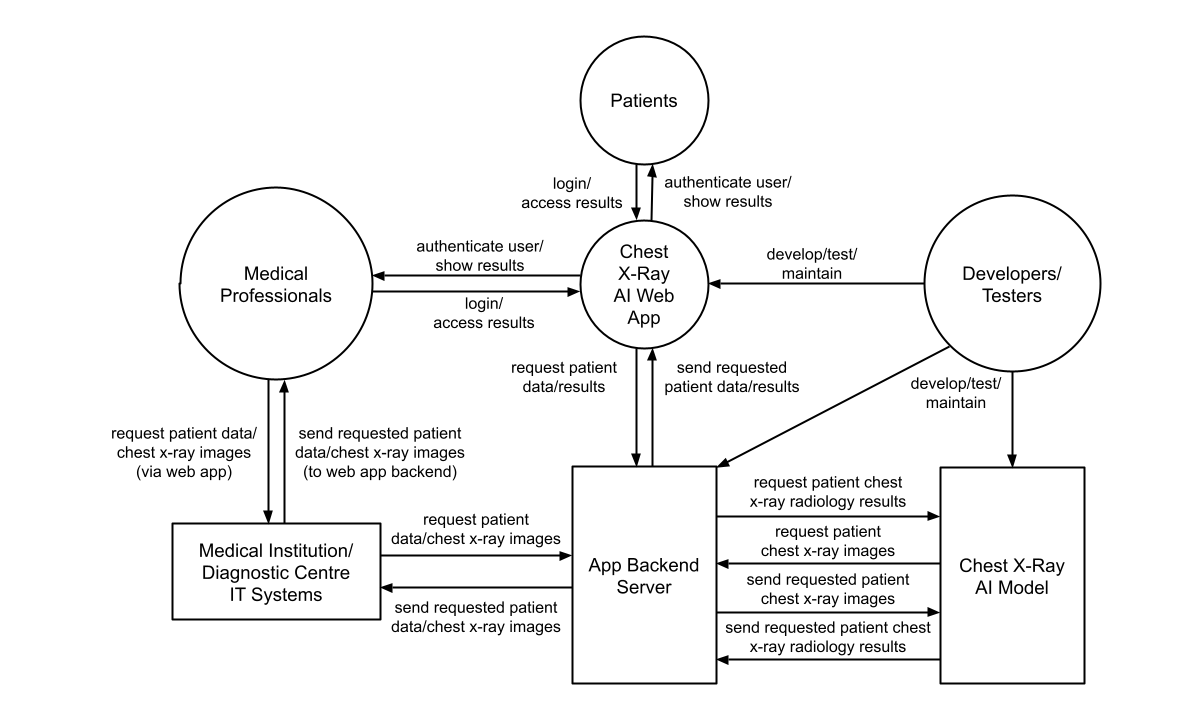
\includegraphics[scale=0.25]{Context Diagram for Chest X-Ray AI Read.png}
    \caption{Context Diagram describing The Context of the Work}
    \label{fig:contextDiagram}
\end{figure}


\subsubsection{Work Partitioning}
The following Tables \ref{tab:workPartitioningEvents} and \ref{tab:workPartitioningSummaries} detail how the work will be partitioned for this project's proposed solution:
\begin{table}[H]
    \centering
    \caption{Work Partitioning Table}
    \label{tab:workPartitioningEvents}
    \begin{tabularx}{\textwidth}{|
    >{\hsize=.6\hsize\linewidth=\hsize}X|>{\hsize=.7\hsize\linewidth=\hsize}X|
    >{\hsize=1.3\hsize\linewidth=\hsize}X|>{\hsize=1.4\hsize\linewidth=\hsize}X|}
        \hline
        \textbf{Event Number} & \textbf{Event Name} & \textbf{Input(s)} & \textbf{Output(s)} \\
        \hline
        1 & Login User & user's login credentials & user's login credentials authenticated \\
        \hline
        2 & Request Patient Data & request for patient data/chest x-ray images & requested patient data/ chest x-ray images \\
        \hline
        3 & Request Radiology Analysis & request for radiology analysis of patient chest x-ray images & radiology report (elements) of the radiology analysis of the patient's chest x-ray images \\
        \hline
        4 & Access/View Radiology Analysis & request to access/ view the radiology results report (elements) & radiology results report (elements) are shown to the user \\
        \hline
        5 & Save Radiology Analysis & request to save the radiology results report (elements) & radiology results report (elements) are saved (to the medical institution's/diagnostic centre's IT systems) \\
        \hline
    \end{tabularx}
\end{table}

\begin{table}[H]
    \centering
    \caption{Work Partitioning Summaries}
    \label{tab:workPartitioningSummaries}
    \begin{tabularx}{\linewidth}{|
    >{\hsize=0.275\hsize\linewidth=\hsize}X|>{\hsize=1.725\hsize\linewidth=\hsize}X|}
        \hline
        \textbf{Event Number} & \textbf{Summary} \\
        \hline
        1 & user enters in login credentials into web app, and web app authenticates the login credentials \\
        \hline
        2 & user requests patient data/chest x-ray images (from medical institution/diagnostic centre IT systems) \\
        \hline
        3 & user requests radiology analysis of patient chest x-ray images \\
        \hline
        4 & user accesses/views resulting radiology report (elements) of the radiology analysis of the patient's chest x-ray images \\
        \hline
        5 & user saves resulting radiology report (elements) of the radiology analysis of the patient's chest x-ray images \\
        \hline
    \end{tabularx}
\end{table}

\subsubsection{Specifying a Business Use Case (BUC)}
The following is a Business Use Case Scenario specified for the project's proposed solution:
\begin{enumerate}
    \item \textbf{Patient arrival:} A patient arrives at the emergency room with severe respiratory symptoms, the attending doctor orders a chest X-ray for assessment of the patient’s lungs.
    \item \textbf{AI chest X-ray:} An X-ray of the patient’s chest is taken and input into the system. The system identifies key abnormalities in the patient.
    \item \textbf{Diagnostic report:} The system generates a list of the identified findings and their severity levels. The user interface presents this information clearly and concisely.
    \item \textbf{Treatment:} The doctor quickly reviews the AI-generated report without examining the X-ray and begins treatment.
\end{enumerate}

\subsection{Business Data Model and Data Dictionary}
\subsubsection{Business Data Model}
The following points detail the business data model of the project's proposed solution:
\begin{itemize}
    \item \textbf{N/A}: this subsection was not filled out, as the details of the business data model will be decided on later in the design and implementation process of the project's proposed solution.
\end{itemize}

\subsubsection{Data Dictionary}
The following points detail the data dictionary of the project's proposed solution:
\begin{itemize}
    \item \textbf{N/A}: this subsection was not filled out, as the details of the data dictionary items will be decided on later in the design and implementation process of the project's proposed solution.
\end{itemize}

\subsection{The Scope of the Product}
This subsection describes the scope of the product, including the product boundary, the product use case table and individual product use cases.

\subsubsection{Product Boundary}
The application encompasses the entire life cycle of the Automated Chest X-ray Diagnosis System, from the initial input of a chest X-ray image to the generation of a structured radiology report. It includes all components such as the Computer Vision and Neural Network modules, User Interface, and Security. 

\subsubsection{Product Use Case Table}
The following table, Table \ref{table:productUseCase}, summarizes the product use cases for the project's proposed solution:
\begin{table}[H]
    \caption{Product Use Case Table}
    \label{table:productUseCase}
    \begin{tabularx}{\textwidth}{|>{\hsize=.4\hsize\linewidth=\hsize}X|>{\hsize=1.6\hsize\linewidth=\hsize}X|}
    \hline
    Use Case ID & Use Case Summary \\
    \hline
    PUC1 & Process chest X-ray image using computer vision module \\
    \hline
    PUC2 & Generate a list of identified findings \\
    \hline
    PUC3 & Convert results into a structured set of findings on the x-ray. \\
    \hline
    PUC4 & Display diagnostic findings on the user interface \\
    \hline
    \end{tabularx}
\end{table}

\subsubsection{Individual Product Use Cases (PUCs)}
The following are the individual product use cases (PUCs), with a description, lists of actors, preconditions and postconditions provided for each.
\begin{enumerate}[label=PUC\arabic*., series=pucs]
    \begin{item}
        \begin{description}
            \item[Description:] the system takes a chest X-ray image as input and processes it to identify abnormalities
            \item[Actors:] computer vision module, chest x-ray image
            \item[Precondition(s):] valid chest x-ray image input is provided
            \item[Postcondition(s):] processed image with identified abnormalities
        \end{description}
    \end{item}
    \begin{item}
        \begin{description}
            \item[Description:] the system generates a comprehensive list of identified findings based on the processed chest X-ray image
            \item[Actors:] computer vision module, neural network module 
            \item[Precondition(s):] processed image with abnormalities is provided
            \item[Postcondition(s):] A list of identified findings is generated 
        \end{description}
    \end{item}
    \begin{item}
        \begin{description}
            \item[Description:] The system converts the list of identified findings into a structured radiology report 
            \item[Actors:] list of findings
            \item[Precondition(s):] A list of identified findings is provided
            \item[Postcondition(s):] diagnostic report is generated
        \end{description}
    \end{item}
    \begin{item}
        \begin{description}
            \item[Description:] The user interface module displays the diagnostic report for the user
            \item[Actors:] user interface module, user
            \item[Precondition(s):] diagnostic report is provided
            \item[Postcondition(s):] diagnostic report is displayed on the user interface
        \end{description}
    \end{item}
\end{enumerate}

\subsubsection{Traceability Matrix}
The following Table \ref{tab:traceabilityMatrix} shows the traceability of each functional requirement to their specific product use cases and vice versa.
\begin{table}[H]
    \centering
    \caption{Traceability Matrix}
    \label{tab:traceabilityMatrix}
    \begin{tabular}{|c|c|c|c|c|}
        \hline
        \diagbox{FR}{PUC} & PUC1 & PUC2 & PUC3 & PUC4 \\
        \hline
        FR1 & X & & & \\
        \hline
        FR2 & & X & & \\
        \hline
        FR3 & & & X & X \\
        \hline
        FR4 & & & & X \\
        \hline
        FR5 & X & X & & \\
        \hline
        FR6 & & & & X \\
        \hline
        FR7 & X & & & \\
        \hline
        FR8 & X & & & \\
        \hline
    \end{tabular}
\end{table}

\subsection{Functional Requirements}
This subsection describes the functional requirements of the project's proposed solution in detail.
It also includes the formal specification description of the machine learning (ML) algorithm to be used in the solution.

\subsubsection{Functional Requirements}
The following are the functional requirements defined for this project's proposed solution. They are described in detail below, with a rationale and fit criterion detailed for each. The individual product use cases associated with each functional requirement are also shown.
\begin{enumerate}[label=FR\arabic*., series=frs]
    \begin{item}
        \begin{description}
            \item[Description:] The system shall accept and read DICOM images as input.
            \item[Rationale:] The model shall use DICOM as the format is easy to process.
            \item[Fit Criterion:] The model can successfully process DICOM files.
            \item[Use Case(s):] PUC1
        \end{description}
    \end{item}
    \begin{item}
        \begin{description}
            \item[Description:] The system shall reject images given in a non-DICOM format.
            \item[Rationale:] The system will process images in a DICOM format and will have no image conversion functionality.
            \item[Fit Criterion:] The system successfully rejects non-DICOM images.
            \item[Use Case(s):] PUC1
        \end{description}
    \end{item}
    \begin{item}
        \begin{description}
            \item[Description:] The system shall display JPEG images in the findings.
            \item[Rationale:] Since the system uses JPEG as input for the model, it is also used to display results.
            \item[Fit Criterion:] The interface is able to map the findings on a JPEG image of the x-ray.
            \item[Use Case(s):] PUC2
        \end{description}
    \end{item}
    \begin{item}
        \begin{description}
            \item[Description:] The system shall generate and display a structured set of findings and demographic information about the patient.
            \item[Rationale:] Displaying a report would help understand the findings of the chest x-ray.
            \item[Fit Criterion:] The system can successfully label the x-rays with the correct diseases normalcy 90\% of the time.
            \item[Use Case(s):] PUC3, PUC4
        \end{description}
    \end{item}
    \begin{item}
        \begin{description}
            \item[Description:] The system shall be able to fetch patients’ records on retrieval request by the user.
            \item[Rationale:] Generated reports and findings need to be accessed in the future when required.
            \item[Fit Criterion:] The system can display the past findings stored in the database.
            \item[Use Case(s):] PUC4
        \end{description}
    \end{item}
    \begin{item}
        \begin{description}
            \item[Description:] \hypertarget{FR5}{The system shall detect and classify the following diseases/infections to a certain accuracy: Pneumonia, Atelectasis, Cardiomegaly, Pleural Effusion}
            \item[Rationale:] Users need information on whether a chest x-ray image depicts any diseases or not.
            \item[Fit Criterion:] The area under the ROC curve for each disease after testing the model is greater than the recommended threshold for accurate results (Refer to Table 6). 
            \item[Use Case(s):] PUC1, PUC2
        \end{description}
    \end{item}
    \begin{item}
        \begin{description}
            \item[Description:] The system shall be accessible remotely via a web interface.
            \item[Rationale:] The database would most likely be on a cloud service, and the system would need to be used remotely from anywhere by the medical professional.
            \item[Fit Criterion:] The interface can retrieve required information from the remote server.
            \item[Use Case(s):] PUC4
        \end{description}
    \end{item}
     \begin{item}
         \begin{description}
             %\item[DELETE?]
             \item[Description:] The system shall convert images from a DICOM file to a jpeg, jpg or other suitable image format to be processed by the ML algorithm.
             \item[Rationale:] Chest x-ray data is stored in DICOM format, and the model uses jpeg images to identify diseases as it is more feasible.
             \item[Fit Criterion:] The system can successfully convert a DICOM x-ray image to a jpeg.
             \item[Use Case(s):] PUC1
             % login page. when login, then browse the list of patients pick one or search using one of the identifiers - name, id and select
             % what landing page should look like
         \end{description}
     \end{item}
    \begin{item}
        \begin{description}
            % build a database - link records to individuals to images
            % database will have patients records and links to images
            \item[Description:] The system shall have a backend database that stores the patient records linked to their diagnostic findings.
            \item[Rationale:] The information should be stored for future access by users.
            \item[Fit Criterion:] User data is stored in a backend database, and can be updated and accessed.
            \item[Use Case(s):] PUC4
        \end{description}
    \end{item}
    \begin{item}
        \begin{description}
            \item[Description:] The system shall allow users to create an account and login.
            \item[Rationale:] Sensitive data needs authorization to be accessed.
            \item[Fit Criterion:] User is able to login through their credentials and access the functions of the system.
            \item[Use Case(s):] PUC2
        \end{description}
    \end{item}
    \begin{item}
        \begin{description}
            \item[Description:] The system shall have a search function to search for diagnoses specific to a patient's details (name, ID, etc)
            \item[Rationale:] Allows fast retrieval of information.
            \item[Fit Criterion:] User is able to search for a patient using their personal information or identifier.
            \item[Use Case(s):] PUC4
        \end{description}
    \end{item}
    % backend models missing
    % add ML model that we will be using - type of model
\end{enumerate}

\begin{table}[H]
    \caption{ROC Threshold Table}
    \label{table:rocTable}
    \begin{tabularx}{\textwidth}{|>{\hsize=1.4\hsize\linewidth=\hsize}X|>{\hsize=.6\hsize\linewidth=\hsize}X|}
    \hline
    Disease/Infection & Expected Area Under ROC Curve\\
    \hline
    Pneumonia & 0.8 \\
    \hline
    Atelectasis & 0.8 \\
    \hline
    Cardiomegaly & 0.85 \\
    \hline
    Pleural Effusion & 0.9 \\
    \hline
    \end{tabularx}
\end{table}

\subsection{Formal Specification for the ML Algorithm}
This subsection details the formal specification for the machine learning algorithm.
The machine learning algorithm can be considered a function (\textit{f}).
The primary output would be to detect \textit{n} different types of diseases.
\begin{gather*}
    f:Image \rightarrow \mathbb{R}^n \\
    f(I) = \{x_i | x_i \in \mathbb{R}; i, n \in \mathbb{N} | 0 \le x_i \le 1, 1 \le i \le n\}
\end{gather*}
 
\noindent Where the input domain is an x-ray image and the output codomain of the function is a vector with \textit{n} dimensions.
Each real number in the vector represents the probability of having a certain disease. 
The report created needs to have a definite prediction (1 or 0) for each disease. The prediction vector is based on whether the probability is above a threshold.  
Suppose each disease has a threshold ($t_i$) for deciding whether the disease is present: 
\begin{align*}
    t_i: \mathbb{R}, 0 \le t_i \le 1, 1 \le i \le n
\end{align*}

\noindent Then the vector constituting the predictions is:
\begin{gather*}
    predictions: \{0,1\}^n \\
    predictions = \Biggl\{ p_i \big| p_i \in \{ 0, 1 \}; i, n, \in \mathbb{N}; x_i \in f(I) \big| 1 \le i \le n, p_i =
    \begin{cases}
        0 & x_i < t_i \\
        1 & x_i \ge t_i
    \end{cases}
    \Biggr\}
\end{gather*}
% it will be conv model, provide some specifics

\section{Non-functional Requirements}
This section covers the various subgroups of non-functional requirements. This includes
look and feel requirements, usability and humanity requirements, performance requirements,
operational and environmental requirements, maintainability and support requirements,
security requirements, cultural requirements and compliance requirements.

\subsection{Look and Feel Requirements}
This subsection details the look and feel requirements of the project's proposed solution.
This encompasses the appearance and style requirements of the solution's user interface.

\subsubsection{Appearance Requirements}
\begin{description}
    \item[NF-AR0] Visual elements shall be consistent, using a clean and intuitive design.
    \begin{description}
        \item[Rationale:] A simple appearance will allow ease of use and minimize complexities from any unintentionally non-intuitive design.
        \item[Fit Criterion:] After one use 80\% of users shall find the design intuitive and visually satisfying.
    \end{description}
\end{description}

\subsubsection{Style Requirements}
\begin{description}
    \item[NF-SR0] The overall style of the user interface shall align with healthcare industry standards and best practices. 
    \begin{description}
        \item[Rationale:] Since the system will be used in medical offices it shall comply with the industry standards to get approval for use.
        \item[Fit Criterion:] The industry standards are met.
    \end{description}
\end{description}

\subsection{Usability and Humanity Requirements}
This subsection details the usability and humanity requirements of the project's proposed solution's user interface:

\subsubsection{Ease of Use Requirements}
\begin{description}
    \item[NF-EUR0] The application interface shall only include the minimum necessary elements for the system to function effectively.
    \begin{description}
        \item[Rationale:] The simplicity of the system is important to ensure that the system is easy for all users to interact with.
        \item[Fit Criterion:] Testers should not be able to identify any element of the user interface that does not serve any immediate and apparent use.
        \item[Traceability:] Traces to functional requirements involving the user interface.
    \end{description}
\end{description}

\subsubsection{Personalization and Internationalization Requirements}
\begin{description}
    \item[NF-PIR0] The interface shall have both official languages of Canada, English and French.
    \begin{description}
        \item[Rationale:] In Canada, people should be able to work in their preferred official language, as per the Official Languages Act(\cite{OLA}).
        \item[Fit Criterion:] The core services shall be available in English and French
    \end{description}
\end{description}

\subsubsection{Learning Requirements}
\begin{description}
    \item[NF-LR0] The interface should be straightforward and easy for all trained hospital or office staff to use.  
    \begin{description}
        \item[Rationale:] The system shall require no training for the use of the interface to allow for smooth integration into the daily activities of the staff.
        \item[Fit Criterion:] During a user's first use of the system, they shall spend no more than 30 seconds reviewing the user interface.
    \end{description}
\end{description}


\subsubsection{Understandability and Politeness Requirements}
\begin{description}
    \item[NF-UPR0] The chest x-ray reports should be coherent and understandable by a radiologist or relevant medical professional. 
    \begin{description}
        \item[Rationale:] The report must be able to outline the findings and any abnormalities determined by the AI model in medical terms with an explanation to be of use to the doctors
        \item[Fit Criterion:] A radiologist or radiologist resident shall be able to comprehend the report findings and justification after reading it once
    \end{description}
\end{description}

\subsubsection{Accessibility Requirements}
\textit{NA}

\subsection{Performance Requirements}
This subsection details the performance requirements of the project's proposed solution:

\subsubsection{Speed and Latency Requirements}
\begin{description}
    \item[NF-SLR0] The system shall return a report generated from an input within a reasonable amount of time. 
    \begin{description}
        \item[Rationale:] The system should be comparable to the time radiologists and residents need to examine a chest X-ray.  
        \item[Fit Criterion:] A report is generated within 5 minutes.
    \end{description}
\end{description}

\subsubsection{Safety-Critical Requirements}
\begin{description}
    \item[NF-SCR0]The system will not collect identifying data not necessary for diagnosis.
    \begin{description}
        \item[Rationale:] Managing all relevant health data for patients requires extra safety measures and puts their data at risk, to minimize the risk all nonessential data will not be collected by the system
        \item[Fit Criterion:] Only data pertaining to diagnosis are collected (X-ray images, age, previous conditions.)
    \end{description}
\end{description}

\subsubsection{Precision or Accuracy Requirements}
\begin{description}
    \item[NF-PAR0] See \hyperlink{FR5}{FR\#5}.
\end{description}

\subsubsection{Robustness or Fault-Tolerance Requirements}
\begin{description}
    \item[NF-RFTR0] The system shall be available 99.7\% of the time, with 30 minutes a week of allowable downtime.
    \begin{description}
        \item[Rationale:] Since the system is aiding in hospital settings, which can run 24/7, offline time should be minimized to allow for the best use of the system.
        \item[Fit Criterion:] The system functions with only 30 minutes of downtime per week of operation.
    \end{description}
\end{description}

\subsubsection{Capacity Requirements}
\begin{description}
    \item[NF-CR0] The system shall be able to receive and process multiple images at a time. 
    \begin{description}
        \item[Rationale:] Multiple patients may require reviews on their chest X-ray at the same point in time and the system should be able to accommodate a small increase in demand. 
        \item[Fit Criterion:] The system shall be able to process 3 or more images at a given time.
    \end{description}
\end{description}

\subsubsection{Scalability or Extensibility Requirements}
\begin{description}
    \item[NF-SER] The system architecture should grow to accommodate an increasing number of chest X-ray images and users as the hospital's workload grows. This is not a concern for this project's current timeline. 
\end{description}


\subsubsection{Longevity Requirements}
\textit{NA}

\subsection{Operational and Environmental Requirements}
This subsection details the operational and environmental requirements for this project's proposed solution:

\subsubsection{Expected Physical Environment}
\begin{description}
    \item[NF-EPE0] The system will be used in hospitals and diagnostic offices. 
    \begin{description}
        \item[Rationale:] This follows from our determined \hyperlink{Users}{stakeholders} for this project and from what the system is built to achieve. 
        \item[Fit Criterion:] \textit{NA}
    \end{description}
\end{description}

\subsubsection{Wider Environment Requirements}
\textit{NA}

\subsubsection{Requirements for Interfacing with Adjacent Systems}
\begin{description}
    \item[NF-RIAS0] The system will require access to the host computer's files for image upload. 
    \begin{description}
        \item[Rationale:] The system requires chest X-ray images to identify any abnormalities in the X-ray, so the system must interface with their computer to facilitate this upload.  
        \item[Fit Criterion:] The user will be able to upload an image from their computer to the system
    \end{description}
\end{description}

\subsubsection{Production Requirements}
\begin{description}
    \item[NF-PR0] The system will be accessible through a web application which requires access to the Internet.  
    \begin{description}
        \item[Rationale:] This allows the system to not be dependent on the type of system currently in-place at hospitals and other medical offices where it could be used. 
        \item[Fit Criterion:] The system can be accessed through a while connected to the Internet. 
    \end{description}
\end{description}

\subsubsection{Release Requirements}
\textit{NA}

\subsection{Maintainability and Support Requirements}
This subsection details the maintainability and support requirements for this project's proposed solution: 

\subsubsection{Maintenance Requirements}
\begin{description}
    \item[NF-MR0] Maintenance of the system will be done by the developers alongside the local IT team.
    \begin{description}
        \item[Rationale:] The developers will work on ensuring the system is working and updated as needed, the local IT team will ensure it's working with the offices existing system. 
        \item[Fit Criterion:] \textit{NA}
    \end{description}
\end{description}

\subsubsection{Supportability Requirements}
\begin{description}
    \item[NF-SR0] The system is self-supporting and will be accompanied by information on the model. 
    \begin{description}
        \item[Rationale:] This allows for less issues with security and dependencies as the system will have all the functionality it needs to operate within it's self.
        \item[Fit Criterion:] The system supports all functionality needed to operate independently. 
    \end{description}
\end{description}

\subsubsection{Adaptability Requirements}
\textit{NA}

\subsection{Security Requirements}
This subsection details the security requirements for this project's proposed solution:

\subsubsection{Access Requirements}
\begin{description}
\hypertarget{AR0}{}
    \item[NF-AR0] The x-ray images should only be accessible to authorized users. Authorized users include doctors and IT staff responsible for storing medical data for the medical institution. 
    \begin{description}
        \item[Rationale:] This is to keep health records confidential and accessible to only those that have permission to view, such as a doctor or nurse. 
        \item[Fit Criterion:] Users with authorized username and password will be able to access the X-ray image.
    \end{description}
    \item[NF-AR1] The system should allow access to generated reports only by medical professionals and the patient to whom the report belongs. 
    \begin{description}
        \item[Rationale:] Similarly to \hyperlink{AR0}{NF-AR0} this is to keep health records confidential and accessible to only those that have permission to view, such as a doctor or nurse. 
        \item[Fit Criterion:] Users with authorized username and password will be able to access the generated report.
    \end{description}
\end{description}


\subsubsection{Integrity Requirements}
\begin{description}
    \item[NF-IR0] The system will encrypt all stored data 
    \begin{description}
        \item[Rationale:] This is to help ensure that if the system is attacked any data is not easily collected. 
        \item[Fit Criterion:] All data is not stored in plain language. 
    \end{description}
\end{description}


\subsubsection{Privacy Requirements}
\begin{description}
    \item[NF-PR0] Only authorized users, doctors, will have access to patients information. 
    \begin{description}
        \item[Rationale:] Similarly to \hyperlink{AR0}{Access requirements} this is to keep records confidential and accessible to only those that have permission to view.
        \item[Fit Criterion:]
    \end{description}
    \item[NF-PR1] The system should maintain the privacy of the patient’s personal and medical information.
    \begin{description}
        \item[Rationale:] This is to follow the medical practices of keeping patient privacy. 
        \item[Fit Criterion:] Patient information is not openly accessible. 
    \end{description}
\end{description}


\subsubsection{Audit Requirements}
\begin{description}
    \item[NF-AR0] Regular security audits and vulnerability assessments shall be conducted to maintain a secure environment. 
    \begin{description}
        \item[Rationale:] This is to ensure that all data is keep private and protected while ensuring that the system is able to provide accurate results for diagnoses. 
        \item[Fit Criterion:] The system maintains a 90\% accuracy rate and authorization safe guards are functioning during an audit.
    \end{description}
\end{description}


\subsubsection{Immunity Requirements}
\textit{NA}


\subsection{Cultural Requirements}
This subsection details the cultural requirements for this project's proposed solution:

\subsubsection{Cultural Requirements}
\begin{description}
    \item[NF-CR0] The system can be used by anyone.
        \begin{description}
        \item[Rationale:] There are many different people living and working in Canada, they should all be able to use the system. 
        \item[Fit Criterion:] All users find the system intuitive and can understand the system after the first use. 
    \end{description}
\end{description}

\subsection{Compliance Requirements}
This subsection details the compliance requirements for this project's proposed solution.

\subsubsection{Legal Requirements}
\begin{description}
    \item[NF-LR0] Patients must consent to the collection of their data and retention of health information must comply with the Person Health Information Protection Act in Canada (\cite{PHIPA}). 
        \begin{description}
        \item[Rationale:] This allows for the system to be able to collect relevant data for diagnosis while operating in Canada. 
        \item[Fit Criterion:] The Person Health Information Protection Act regulations are followed. 
    \end{description}
\end{description}

\subsubsection{Standards Compliance Requirements}
\begin{description}
    \item[NF-SCR0] The system shall comply with the Canadian healthcare standards. 
        \begin{description}
        \item[Rationale:] Since the system will be used within medical centres for diagnostics it is considered a software medical technology and to be used in hospitals it must meet the standards. 
        \item[Fit Criterion:] The standards are met. 
    \end{description}
\end{description}

\section{Project Issues}
This section covers the various project issues, namely open issues, off-the-shelf solutions,
new problems, tasks, migration to the new product, costs, waiting room and ideas for solutions.

\subsection{Open Issues}
\begin{itemize}
    \item \textbf{Algorithm Optimization:} The optimization of algorithms for the computer vision and neural network modules require further exploration to enhance the efficiency and accuracy of chest X-ray analysis.
    \item \textbf{Web Application Dependency:} The dependency on a web application for system functionality may pose challenges in environments with restricted internet access.
    \item \textbf{Data Security Measures:} The implementation of robust security measures to protect patient information requires careful consideration and potential enhancements.
\end{itemize}

\subsection{Off-the-Shelf Solutions}

\subsubsection{Ready-Made Products}
\begin{itemize}
    \item \textbf{Deep Learning Frameworks:} Leveraging existing deep learning such as PyTorch or TensorFlow to accelerate the development and optimization of the computer vision and neural network modules.
    \item \textbf{User Interface Libraries:} Utilizing established user interface libraries like React or Angular to expedite the development of the user interface component.
\end{itemize}
\subsubsection{Reusable Components}
N/A
\subsubsection{Products That Can Be Copied}
\begin{itemize}
    \item \textbf{Web Application Frameworks:} Identifying web application frameworks (i.e. Django, Ruby, ExpressJS) that align with the project's requirements to serve as a foundation for the system.
\end{itemize}

\subsection{New Problems}

\subsubsection{Effects on the Current Environment}
\begin{itemize}
    \item Introduction of this technology may lead to an over-reliance, potentially diminishing the role of traditional diagnostic methods. 
    \item In the event of software malfunction, there is a risk of significant delays, surpassing current delay times. 
\end{itemize}
\subsubsection{Effects on the Installed Systems}
    N/A
\subsubsection{Potential User Problems}
\begin{itemize}
    \item Some radiologists and healthcare professionals may exhibit skepticism toward adopting this technology.
    \item There is a risk of user error, such as unintentional submission of non-X-ray images. 
\end{itemize}
\subsubsection{Limitations in the Anticipated Implementation Environment That May
Inhibit the New Product}
\begin{itemize}
    \item The system is designed to process only one image at a time, potentially hindering workflow efficiency in scenarios where batch processing is desired. 
    \item A functional web application is needed to run the software. 
\end{itemize}
\subsubsection{Follow-Up Problems}
    N/A

\subsection{Tasks}

\subsubsection{Project Planning}
% \begin{itemize}
%     \item \textbf{September 25th, 2023}: Problem Statement and Goals
%     \item \textbf{September 25th, 2023}: Development Plan
%     \item \textbf{October 4th, 2023}: Requirements Document, Revision 0
%     \item \textbf{October 20th, 2023}: Hazard Analysis, Revision 0
%     \item \textbf{November 3rd, 2023}: V\&V Plan, Revision 0
%     \item \textbf{November 13th – 24th, 2023}: Proof of Concept Demonstration
%     \item \textbf{January 17th, 2024}: Design Document, Revision 0
%     \item \textbf{February 5th – 16th, 2024}: Revision 0 Demonstration
%     \item \textbf{ March 6th, 2024}: V\&V Report, Revision 0
%     \item \textbf{March 18th – 29th, 2024}: Final Demonstration, Revision 1
%     \item \textbf{April TBD}: EXPO Demonstration
%     \item \textbf{April 4th, 2023}: Final Documentation, Revision 1
% \end{itemize}

    \begin{center}
    \begin{tabular}{ |c|c| } 
    \hline
    \textbf{Deliverable} & \textbf{Deadline} \\ 
    \hline
    Problem Statement and Goals, Development Plan & September 25th, 2023 \\ 
    Requirements Document, Revision 0  & October 6th, 2023 \\
    Hazard Analysis, Revision 0 & October 20th, 2023  \\ 
    V\&V Plan, Revision 0 & November 3rd, 2023 \\ 
    Proof of Concept Demonstration & November 13th - 24th, 2023 \\
    Design Document, Revision 0 & January 17th, 2023 \\
    Revision 0 Demonstration & February 5th - February 16th, 2024\\
    V\&V Report, Revision 0 & March 6th, 2024 \\
    Final Demonstration, Revision 1 & March 18th - March 29th, 2024 \\
    EXPO Demonstration & April TBD \\
    Final Documentation, Revision 1 & April 4th, 2024 \\
    \hline
    \end{tabular}
    \end{center}

\subsubsection{Planning of the Development Phases}

    \begin{enumerate}
      \item \textbf{Initiation Phase} (September 5th, 2023 - September 25th, 2023)
      \begin{itemize}
        \item Team building and project selection.
        \item Identify the project supervisor.
        \item Create a \textit{GitHub} project repository.
      \end{itemize}
    
      \item \textbf{Planning Phase} (September 26th, 2023 - October 11th, 2023)
      \begin{itemize}
        \item Create a Development Plan.
        \item Define the problem and scope of the project.
        \item Identify stakeholders and investigate their needs.
        \item Create SRS Documentation.
      \end{itemize}
    
      \item \textbf{First Implementation Phase} (October 12th, 2023 - November 24th, 2023)
      \begin{itemize}
        \item Address the implementation challenges of the project.
        \item Perform Hazard Analysis.
        \item Create the Verification and Validation Plan.
        \item Present Proof of Concept Demonstration.
      \end{itemize}
      
      \item \textbf{Second Implementation Phase} (November 25th, 2023 - January 17th, 2024)
      \begin{itemize}
        \item Implement the main features of the project.
        \item Perform testing.
        \item Optimize the implementation details of the project.
        \item Create the Design Document (Version 0).
      \end{itemize}
    
      \item \textbf{Evaluation Phase} (January 18th, 2024 - March 6th, 2024)
      \begin{itemize}
        \item Evaluate the achievement of project goals.
        \item Perform risk and security assessments.
        \item Conduct user-end testing assessments.
        \item Demonstrate Revision 0.
        \item Prepare the Verification and Validation Report.
      \end{itemize}
    
      \item \textbf{Closure Phase} (March 7th, 2024 - April 4th, 2024)
      \begin{itemize}
        \item Conduct the final demonstration.
        \item Get ready for the Expo Demonstration.
        \item Complete all documentation.
      \end{itemize}
    \end{enumerate}

\subsection{Migration to the New Product}

\subsubsection{Requirements for Migration to the New Product}
N/A
\subsubsection{Data That Has to be Modified or Translated for the New System}
N/A

\subsection{Costs}
There are no costs anticipated with this project, however, should any purchases be necessary the total will not exceed \$750.

\subsection{User Documentation and Training}
This subsection contains the details of all needed user documentation and training for this project's proposed solution.

\subsubsection{User Documentation Requirements}
The system will have the following documentation provided to the users:
\begin{description}
    \item[User Interface:] The system will have a guide outlining the use of each section of the UI and accepted forms on data that can be uploaded to the system.  
    \item[Model:] The model is more complex and will come with details pertaining to the accuracy of detection, which diseases the system can identify, the policy of storing and keeping information, and maintenance and updates.
\end{description}


\subsubsection{Training Requirements}
There will be no training requirements.


\subsection{Waiting Room}
N/A

\subsection{Ideas for Solution}
N/A

\bibliographystyle{plainnat}
\bibliography{SRS, PHIPA, OLA}

\newpage{}
\section{Appendix}

\subsection{Reflection}
The information in this section will be used to evaluate the team members on the
graduate attribute of Lifelong Learning.  Please answer the following questions:

\begin{enumerate}
  \item What knowledge and skills will the team collectively need to acquire to
  complete this capstone project?  Examples of possible knowledge
  to acquire include domain-specific knowledge from the domain of your
  application, software engineering knowledge, mechatronics knowledge or
  computer science knowledge.  Skills may be related to technology, writing,
  presentation, team management, etc.  You should look to identify at
  least one item for each team member.
  \item For each of the knowledge areas and skills identified in the previous
  question, what are at least two approaches to acquiring the knowledge or
  mastering the skill?  Of the identified approaches, which will each team
  member pursue, and why did they make this choice?
\end{enumerate}

The main skills that the team shall collectively aim to learn through this project are documentation, version control and management of group work using GitHub, and project specific knowledge such as computer vision/machine learning. The team aims to learn about machine learning by reading various research papers about chest x-ray disease detection. There are also skills that different team members aim to learn individually through this project.

For documentation, version control, and GitHub management, the team plans to adopt a hands-on approach by actively engaging in a collaborative projects, leveraging GitHub for version control, and documenting their progress consistently. To delve into computer vision and machine learning, the team aims to combine theoretical understanding with practical implementation. They will explore online courses, tutorials, and community forums to grasp foundational concepts, while simultaneously working on the chest X-ray disease detection project to apply this knowledge in a real-world context. Each team member will choose the approach that aligns with their preferred learning style, some might favor structured courses while others opt for self-directed exploration. This diversity in learning approaches ensures a comprehensive understanding of the subjects. 



\end{document}